%!TEX program = xelatex
% \documentclass{beamer}
\documentclass[aspectratio=169]{beamer}

% \usepackage[english]{babel}

% \usepackage{graphicx,hyperref,url, materialbeamer}
% \usepackage{braket}
% \usepackage{euler}
% \usepackage{listings}

\usepackage{materialbeamer}

% \graphicspath{ {../Images/} }
\setbeamercovered{transparent}
\lstdefinestyle{customsql}{
  belowcaptionskip=1\baselineskip,
  breaklines=true,
  xleftmargin=\parindent,
  language=SQL,
  showstringspaces=false,
  basicstyle=\footnotesize\ttfamily,
  keywordstyle=\bfseries\color{green!40!black},
  commentstyle=\itshape\color{purple!40!black},
  identifierstyle=\color{blue},
  stringstyle=\color{orange},
}
\lstset{escapechar=@,style=customsql}
\usefonttheme{professionalfonts} % using non standard fonts for beamer

% The title of the presentation:
%  - first a short version which is visible at the bottom of each slide;
%  - second the full title shown on the title slide;
% Todo: Fill your thesis title
\title[Diploma Thesis]{Example Thesis Title}

% Optional: a subtitle to be displayed on the title slide
\subtitle{Diploma Thesis}

% The author(s) of the presentation:
%  - again first a short version to be displayed at the bottom;
%  - next the full list of authors, which may include contact information;
% \author[L. Lancia \& G. Salillari]{L. Lancia, G. Salillari}
% Todo: Fill you full name
\author{Surname Name}

% Todo: Position logo in respect to your title
% set the y parameter in the \put(175, y) (in this example it is set 30)
\titlegraphic{
  \begin{picture}(0,0)
    \put(175,30){\makebox(0,0)[rt]{
\includegraphics[width=3cm]{../Images/TUC_logo_circle.png}}}
  \end{picture}
}

% The institute:
%  - to start the name of the university as displayed on the top of each slide
%    this can be adjusted such that you can also create a Dutch version
%  - next the institute information as displayed on the title slide
\institute[Technical University of Crete]{Electrical \& Computer Engineering School\\Technical University of Crete}

% Add a date and possibly the name of the event to the slides
%  - again first a short version to be shown at the bottom of each slide
%  - second the full date and event name for the title slide
\date[\today]{\today}

% \providecommand{\di}{\mathop{}\!\mathrm{d}}
% \providecommand*{\der}[3][]{\frac{d\if?#1?\else^{#1}\fi#2}{d #3\if?#1?\else^{#1}\fi}}
%  \providecommand*{\pder}[3][]{%
%     \frac{\partial\if?#1?\else^{#1}\fi#2}{\partial #3\if?#1?\else^{#1}\fi}%
%   }
\begin{document}

\begin{frame}
	\titlepage
\end{frame}

\begin{frame}{Table of Contents}
	\tableofcontents
\end{frame}

\chapter{Introduction}
\label{Chapter-Introduction}

\section{Motivation}
\section{Scientific Contributions}
\section{Thesis Outline}
% Todo: fill chapter descriptions
\begin{itemize}
	\item \textbf{Chapter 2 - Theoretical Background:} Chapter 2 description
	\item \textbf{Chapter 3 - Related Work:} Chapter 3 description
	\item \textbf{Chapter 4 - Robustness Analysis:} Chapter 4 description
	\item \textbf{Chapter 5 - FPGA Implementation:} Chapter 5 description
	\item \textbf{Chapter 6 - Results:} Chapter 6 description
	\item \textbf{Chapter 7 - Conclusions and Related Work:} Chapter 7 description
\end{itemize}

\chapter{Theoretical Background}
\label{Chapter-Theoretical-Background}

% Todo: Edit to your liking
\section{Subject A}
\section{Subject B}

\section{Theoretical knowledge sources}

\chapter{Related Work}
\label{Chapter-Related-Work}

% Todo: edit to your liking
\section{Related work A}
\section{Related work B}

\section{The FPGA Perspective}
\section{Thesis Approach}

\chapter{Robustness Analysis}
\label{Chapter-Robustness-Analysis}

% Todo: edit to your liking
\section{Experiment A}
\section{Experiment B}

\setlength{\parskip}{\baselineskip}
\section{Architecture Design}

\begin{frame}
	\huge Architecture Design
\end{frame}

% Todo: Edit to your liking
\begin{frame}{Some Title}
	\begin{itemize}
		\item Some item 1
		\item Some item 2
		\item Some item 3
	\end{itemize}
\end{frame}

\setlength{\parskip}{\baselineskip}
\section{FPGA Implementation}

\begin{frame}
    \huge FPGA Implementation
\end{frame}

% Use as a reference - Edit to your liking

% Todo: Replace with your platform
\begin{frame}{Xilinx ZCU102 Evaluation Kit}
	\centering
	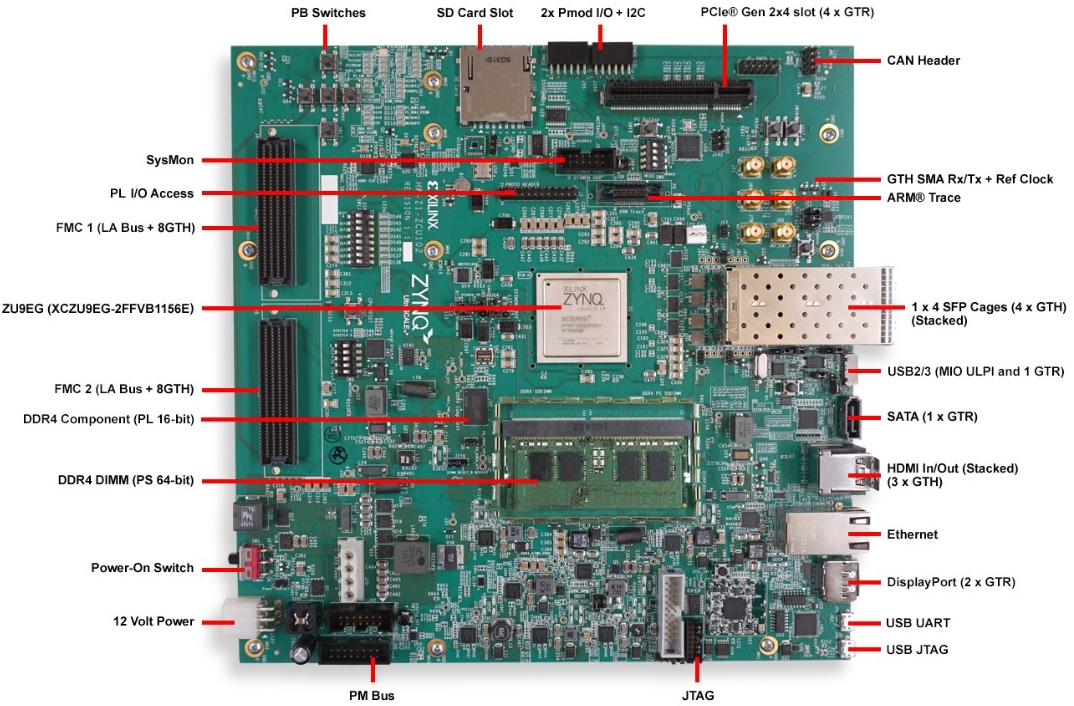
\includegraphics[width=0.65\textwidth]{../Images/Hardware/ZCU102-board-overview.jpg}\\
\end{frame}

% Todo: Replace with your toolchain
\begin{frame}{Tools Used: Xilinx Vivado HLS}
	\begin{minipage}{0.6\textwidth}
		\centering
		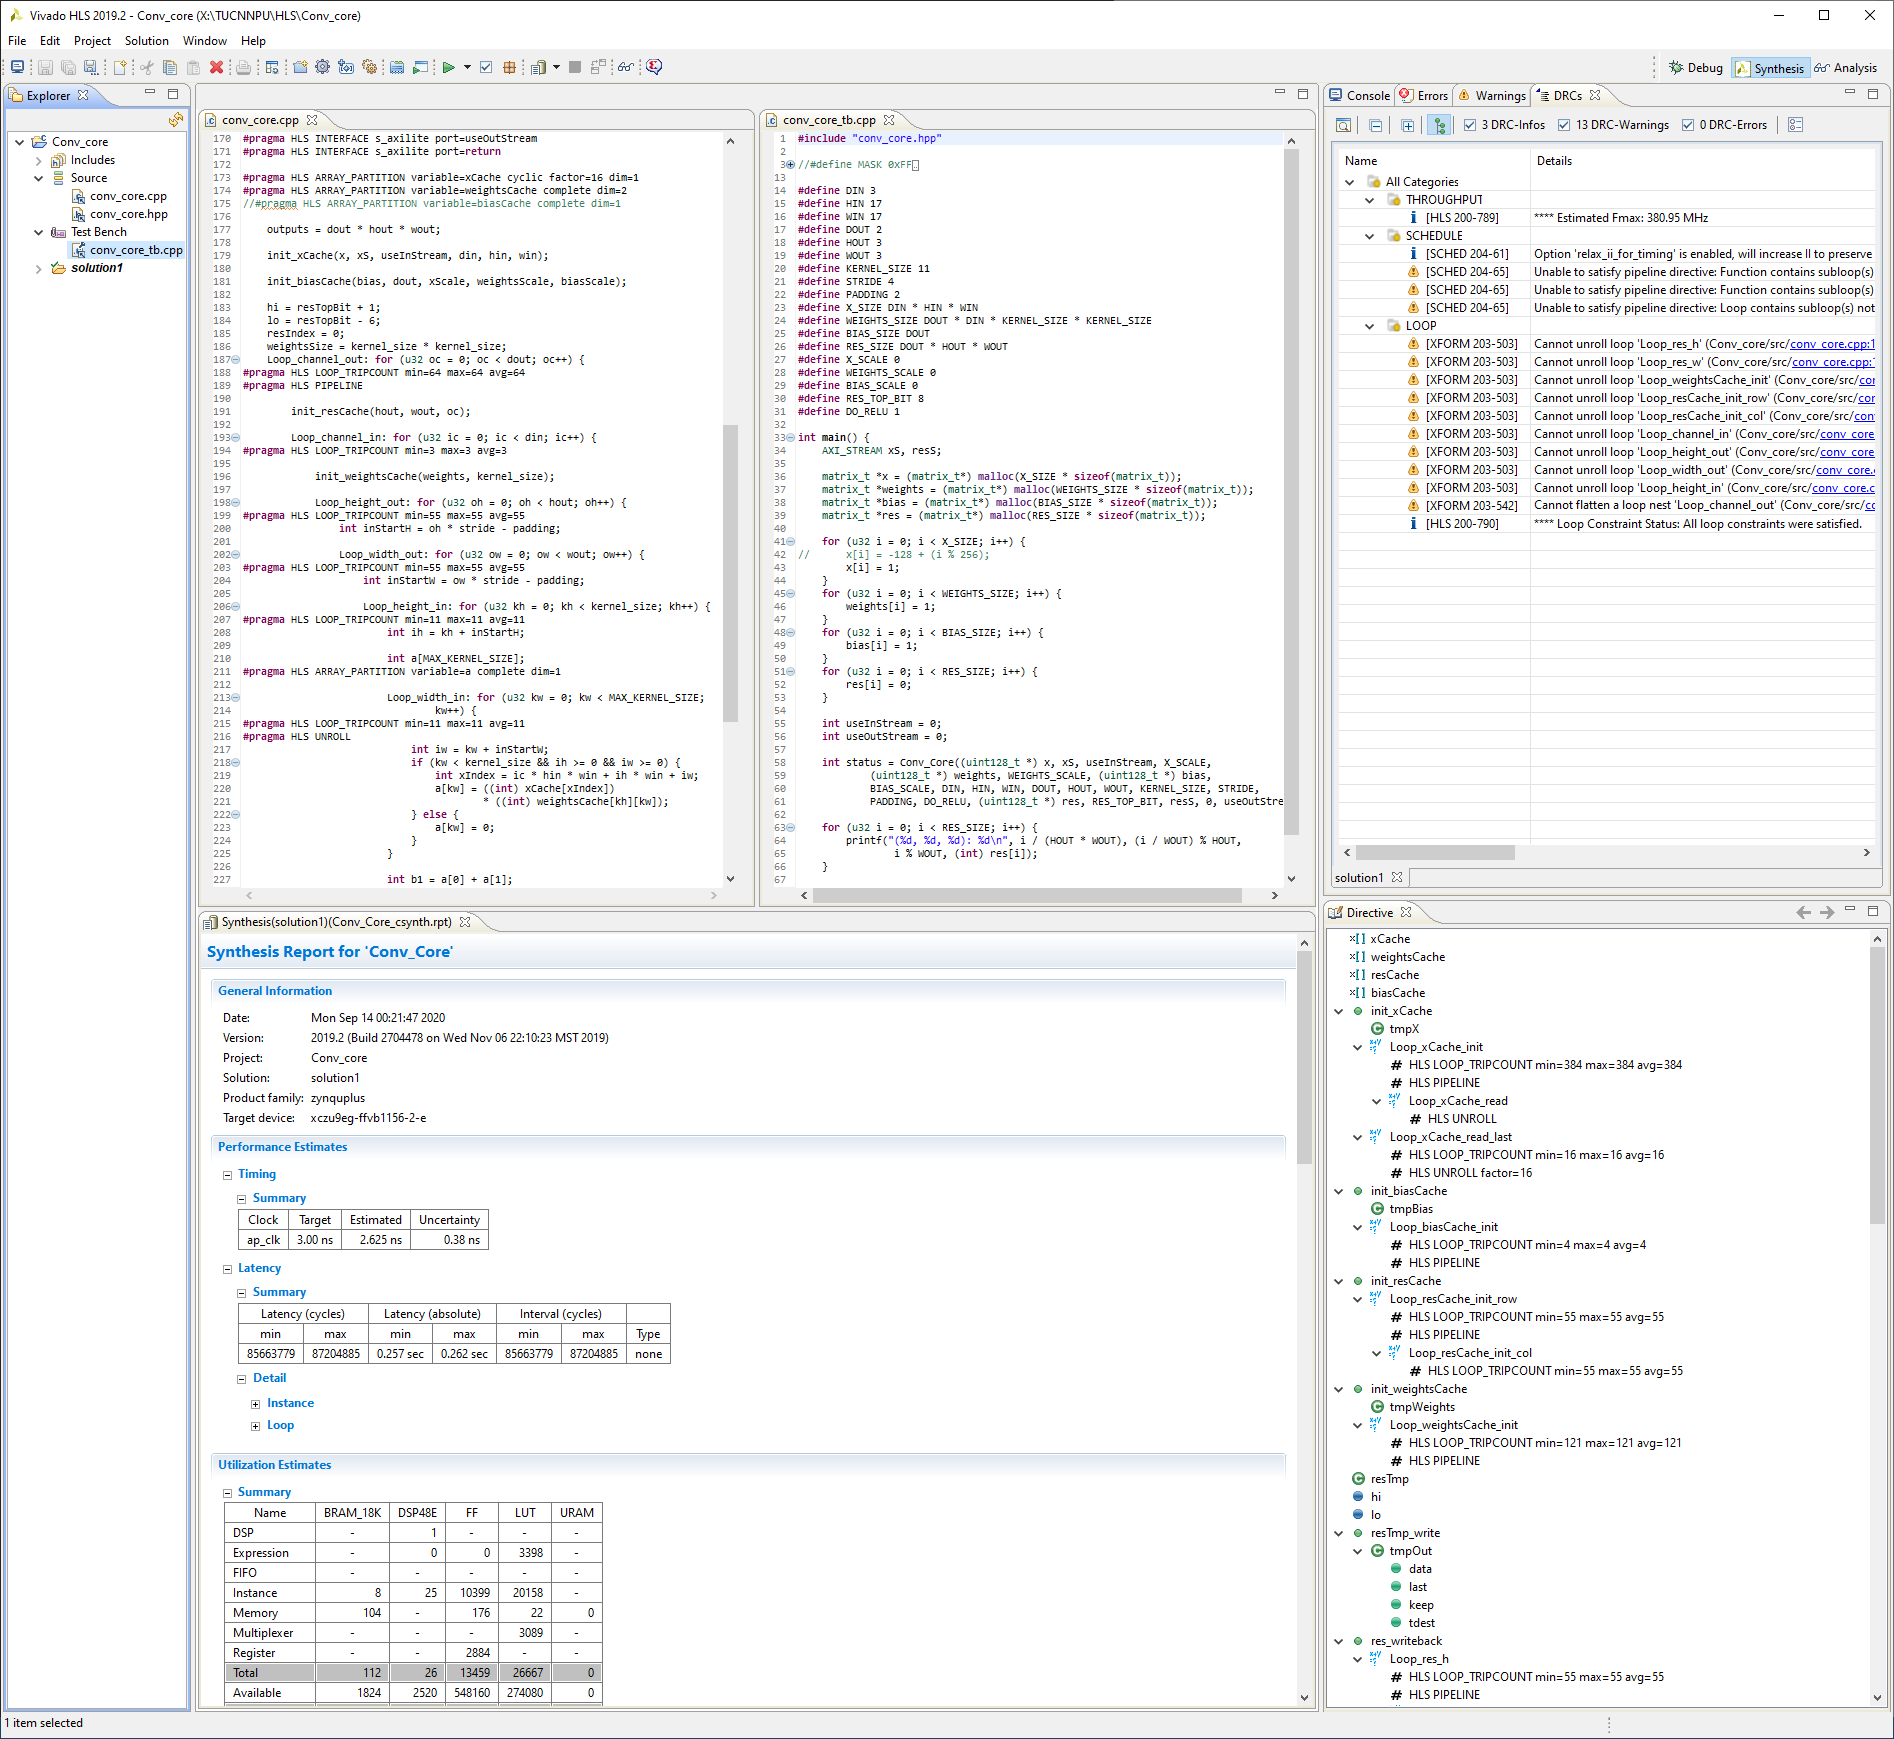
\includegraphics[width=0.8\textwidth]{../Images/Platform/Vivado-HLS.png}\\
	\end{minipage}%
	\begin{minipage}{0.4\textwidth}
		\begin{itemize}
			\item Now Vitis HLS
			\item High-level design using C/C++, SystemC, OpenCL
			\item Generates VHDL \& Verilog HDL designs
			\item Directives
			\item C/C++ testbench
			\item C/RTL Cosimulation
			\item Synthesis Report
		\end{itemize}
	\end{minipage}
\end{frame}

\begin{frame}{Tools Used: Xilinx Vivado IDE}
	\begin{minipage}{0.6\textwidth}
		\centering
		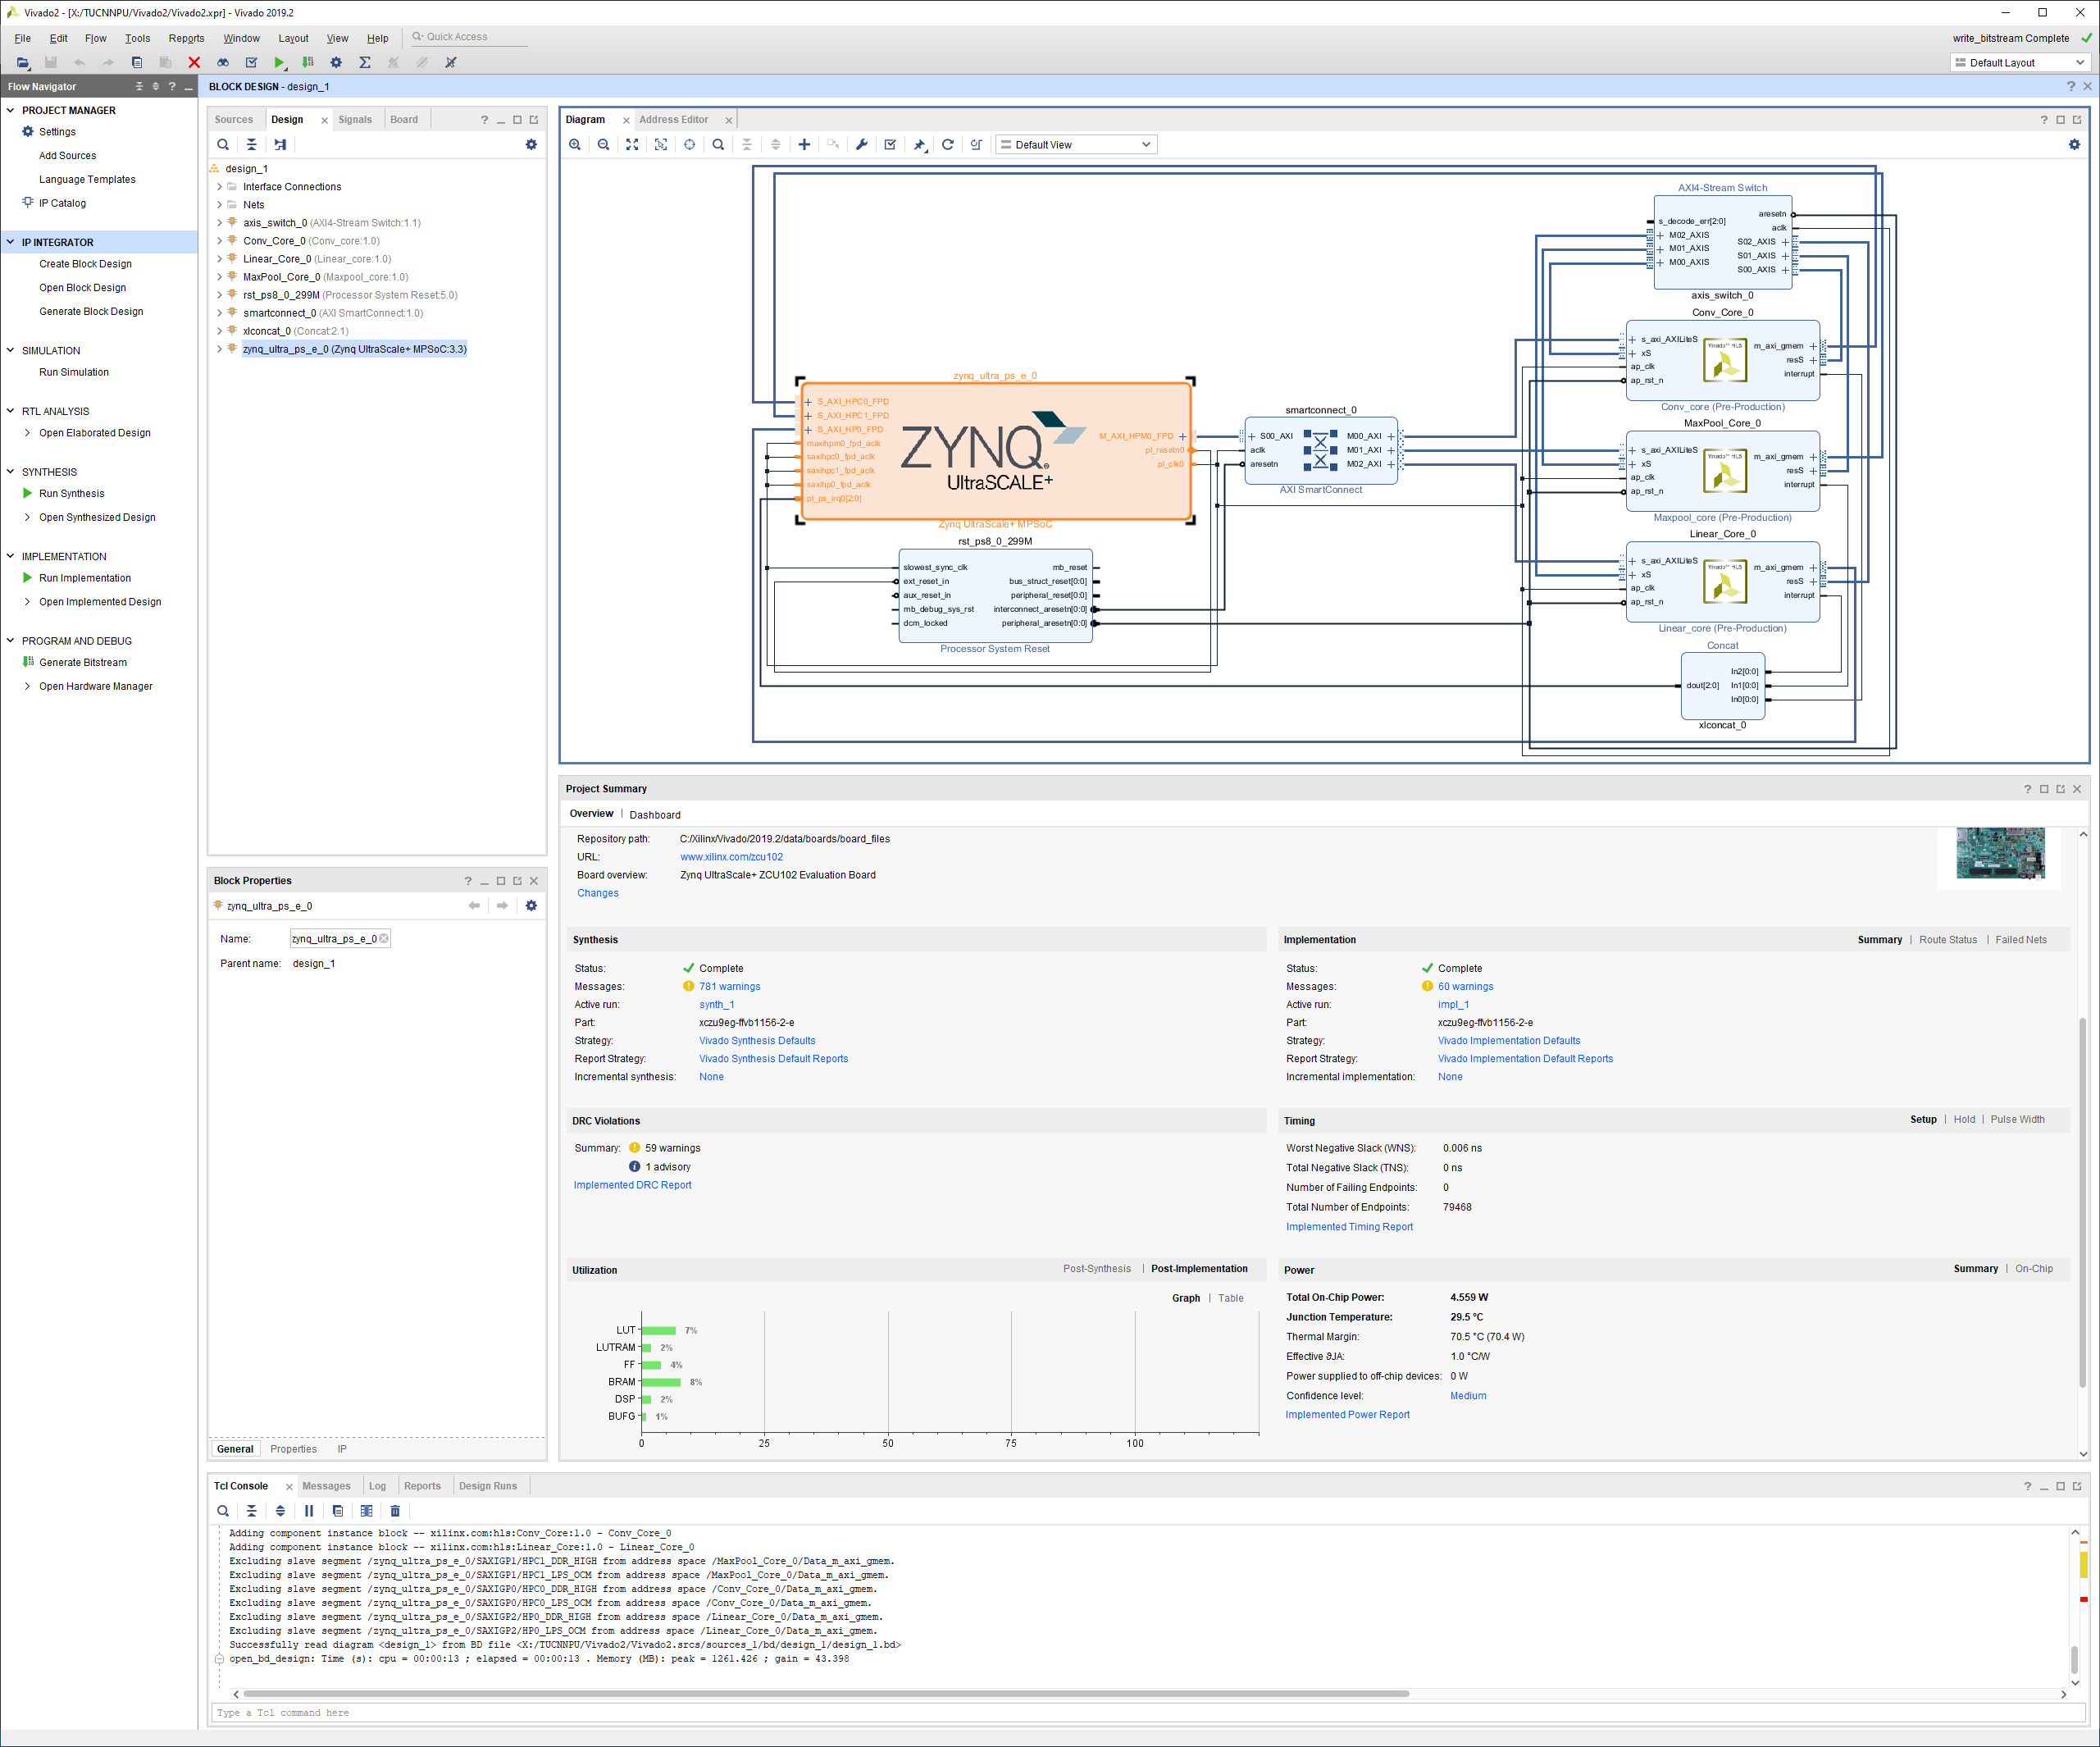
\includegraphics[width=0.9\textwidth]{../Images/Platform/Vivado-IDE.png}\\
	\end{minipage}%
	\begin{minipage}{0.4\textwidth}
		\begin{itemize}
			\item VHDL \& Verilog
			\item IP Integrator Tool
			\item Vivado HLS RTL designs
			\item Synthesis, Implementation \& Download RTL designs
			\item RTL Simulators \& Integrated Logic Analyzer IPs
		\end{itemize}
	\end{minipage}
\end{frame}

\begin{frame}{Tools Used: Xilinx SDK/Vitis IDE}
	\begin{minipage}{0.6\textwidth}
		\centering
		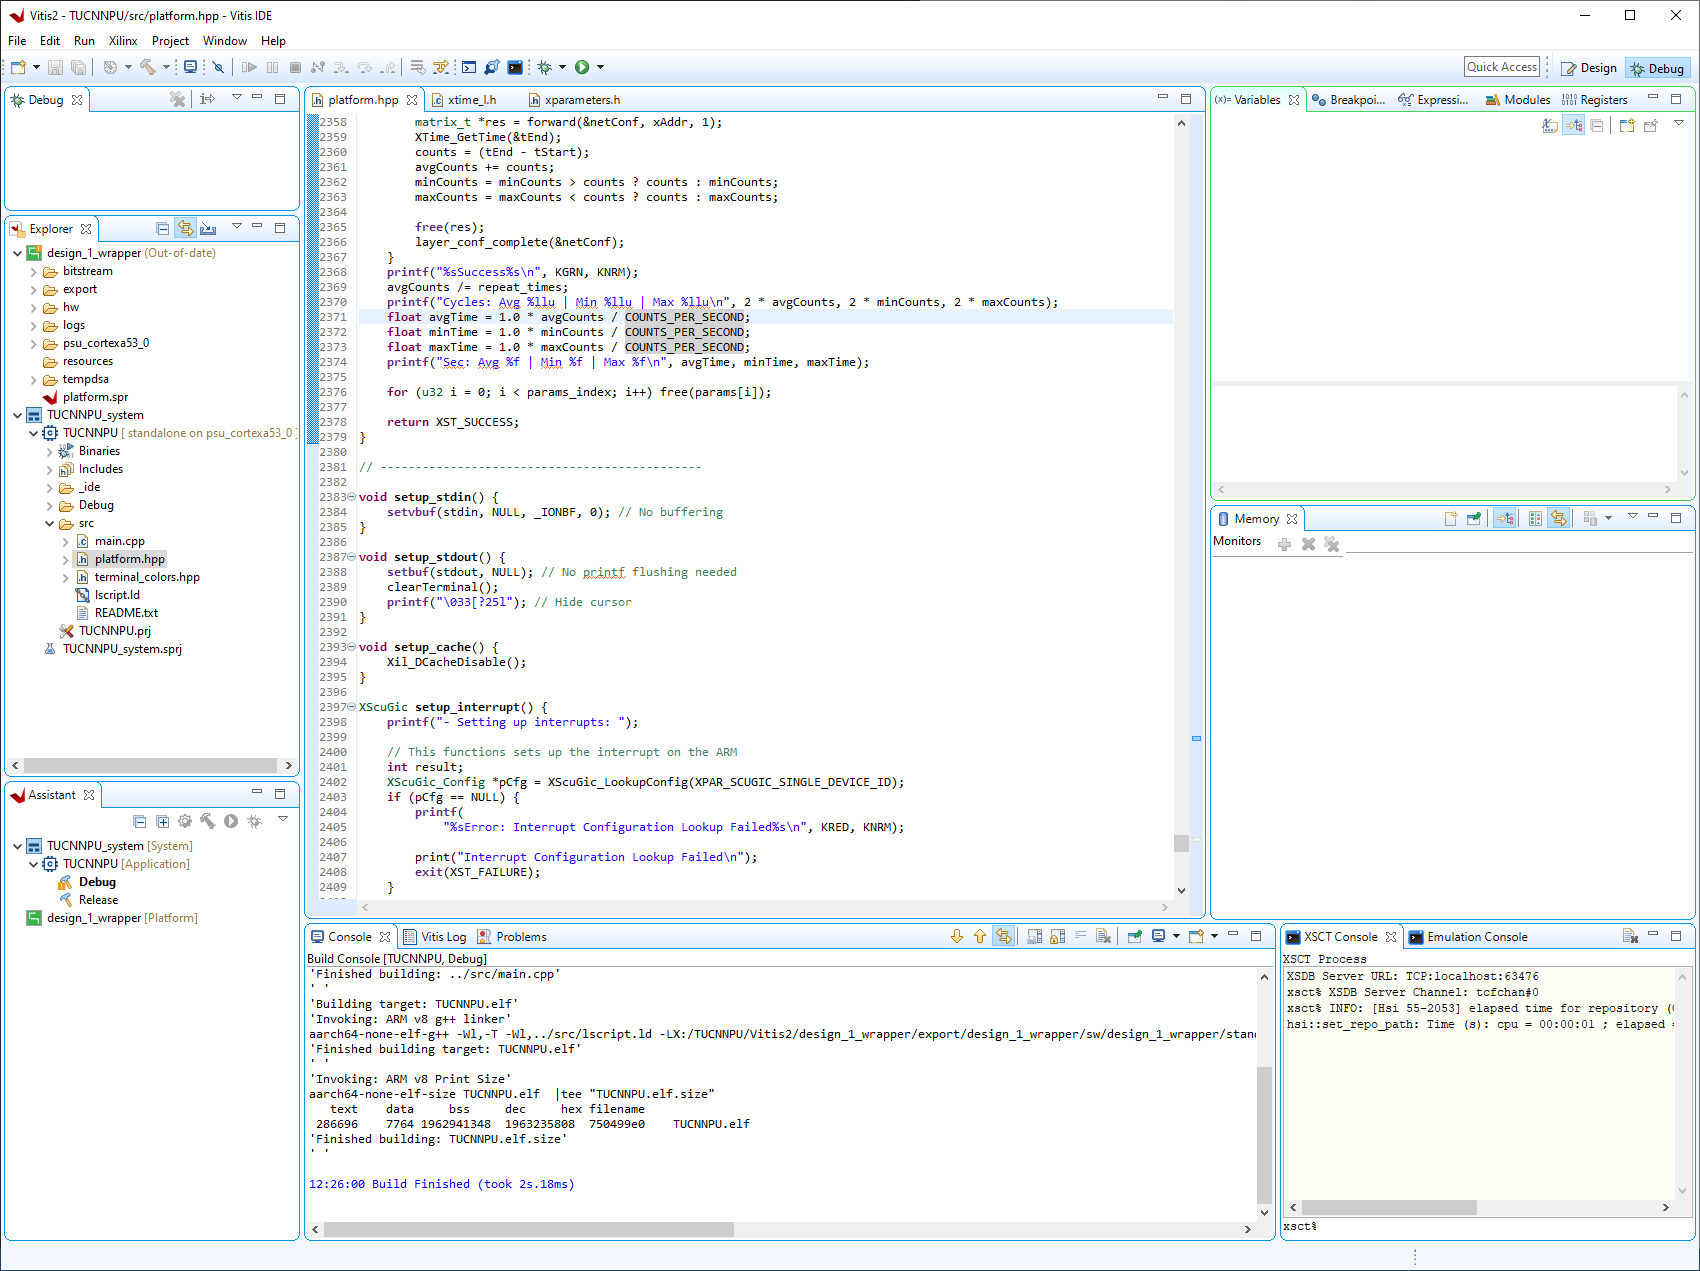
\includegraphics[width=\textwidth]{../Images/Platform/Vitis-IDE.png}\\
	\end{minipage}%
	\begin{minipage}{0.4\textwidth}
		\begin{itemize}
			\item Vitis IDE  integrates SDK, SDAccel, SDSoC tools
			\item C/C++ IDE
			\item Application development for PS part
			\item PetaLinux \& FreeRTOS
			\item Download bitstreams
			\item Debugging tools
		\end{itemize}
	\end{minipage}
\end{frame}

\setlength{\parskip}{\baselineskip}
\section{Results}

\begin{frame}
	\huge Results
\end{frame}

% Todo: Fill information
\begin{frame}{Compared Platforms: CPU}
	\center{\large{Some CPU model}}
	\begin{table}[H]
		\centering
		\begin{tabular}{ll}
			\toprule
			\textbf{Cores / Threads}      & x/x      \\
			\textbf{Max Turbo Frequency}  & x GHz   \\
			\textbf{TDP}                  & x W      \\
			\textbf{Max Memory Bandwidth} & x GB/s \\
			\textbf{Lithography}          & x nm     \\
			\bottomrule
		\end{tabular}
	\end{table}
\end{frame}

% Todo: Fill information
\begin{frame}{Compared Platforms: GPU}
	\center{\large{Some GPU model}}
	\begin{table}[H]
		\centering
		\begin{tabular}{ll}
			\toprule
			\textbf{CUDA Cores}        & x      \\
			\textbf{Tensor Cores}      & x        \\
			\textbf{GPU Memory}        & x GB GDDR6 \\
			\textbf{Boost Clock}       & x MHz  \\
			\textbf{Memory Interface}  & x-bit   \\
			\textbf{Memory Bandwidth}  & x GB/s   \\
			\textbf{Power Consumption} & x W      \\
			\bottomrule
		\end{tabular}
	\end{table}
\end{frame}

% Todo: Fill information
\begin{frame}{Compared Platforms: FPGA}
	\center{\large{Some FPGA Platform}}
	\begin{table}[H]
		\centering
		\begin{tabular}{ll}
			\toprule
			\textbf{PL/DSP Clock Frequency} & x/x MHz \\
			\textbf{LUT Usage}              & x\%      \\
			% 		\textbf{LUTRAM Usage} & -\\
			\textbf{FF Usage}               & x\%     \\
			\textbf{BRAM Usage}             & x\%     \\
			\textbf{DSP Usage}              & x\%     \\
			% 		\textbf{BUFG Usage} & -\\
			\bottomrule
		\end{tabular}
	\end{table}
\end{frame}

% Todo: Fill information
\begin{frame}{Compared Platforms: FPGA}
	\center{\large{Proposed Platform}}
	\begin{table}[H]
		\centering
		\begin{tabular}{ll}
			\toprule
			\textbf{Clock Frequency (MHz)} & xMHz \\
			\textbf{LUT Usage}             & x\% \\
			\textbf{LUTRAM Usage}          & x\% \\
			\textbf{FF Usage}              & x\% \\
			\textbf{BRAM Usage}            & x\% \\
			\textbf{DSP Usage}             & x\%  \\
			% \textbf{BUFG (\%)}             & x\% \\
			\bottomrule
		\end{tabular}
	\end{table}
\end{frame}

% Todo: Fill configuration information
\begin{frame}{CPU \& GPU Performance}
	\begin{itemize}
		\item Config 1
		\item Config 2
		\item Config 3
	\end{itemize}
\end{frame}

% Todo: Replace graph
\begin{frame}{CPU \& GPU Performance: Latency}
	\centering
	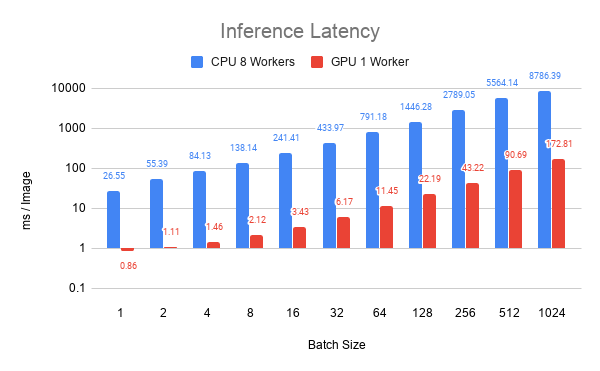
\includegraphics[width=0.7\textwidth]{../Images/Results/CPU-GPU-Inference-Latency.png}\\
\end{frame}

% Todo: Replace graph
\begin{frame}{CPU \& GPU Performance: Throughput}
	\centering
	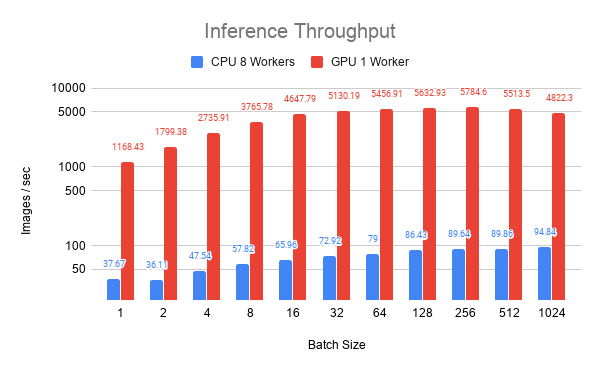
\includegraphics[width=0.7\textwidth]{../Images/Results/CPU-GPU-Inference-Throughput.png}\\
\end{frame}

% Todo: Fill information
\begin{frame}{Final Performance}
	\begin{table}[H]
		\centering
		\begin{tabular}{l|l|l|l|l}
			\toprule
			                                    & \textbf{CPU} & \textbf{GPU} & \textbf{CHaiDNN} & \textbf{Proposed Platform} \\
			\midrule
			\textbf{Clock Frequency (MHz)}      & x				& x				& x					& x							\\
			\textbf{Throughput (Images/s)}      & x				& x				& x					& x							\\
			\textbf{Throughput Speedup}         & 100\%			& x\%			& x\%				& x\%						\\
			\textbf{Latency (s)}                & x				& x				& x					& x							\\
			\textbf{Latency Speedup}            & 100\%			& x\%			& x\%				& x\%						\\
			\textbf{Total On-Chip Power (Watt)} & x				& x				& x					& x							\\
			\textbf{Power Efficiency}           & 100\%			& x\%			& x\%				& x\%						\\
			\textbf{Energy Cons./Image (Joule)} & x				& x				& x					& x							\\
			\textbf{Energy Efficiency}          & 100\%			& x\%			& x\%				& x\%						\\
			\textbf{Images/Joule}               & x				& x				& x					& x							\\
			\bottomrule
		\end{tabular}
	\end{table}
\end{frame}

% Todo: Replace graph
\begin{frame}{Final Performance}
	\centering
	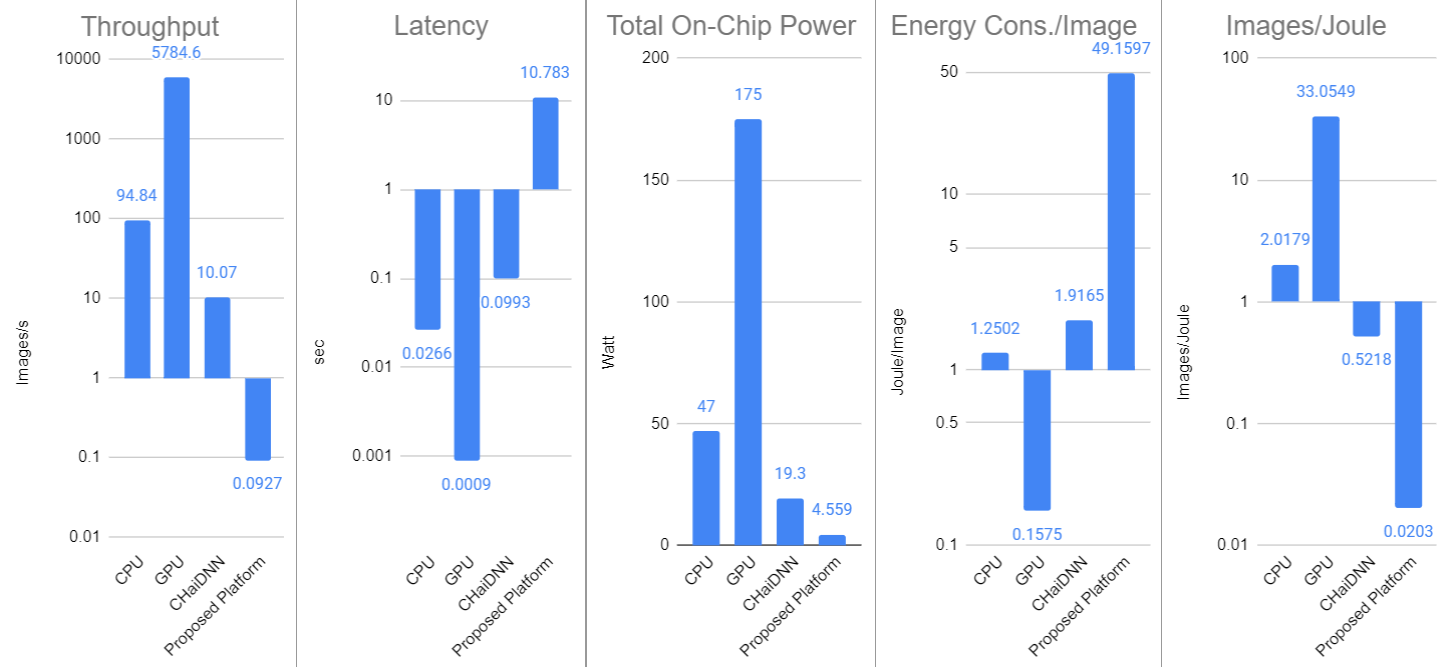
\includegraphics[width=0.9\textwidth]{../Images/Results/Final-Results-charts.png}\\
\end{frame}

\setlength{\parskip}{\baselineskip}
\section{Conclusion}

\begin{frame}
	\huge Conclusions \& Future Work
\end{frame}

% Todo: Edit to your liking
\begin{frame}{Conclusions}
	\begin{itemize}
		\item Conclusion 1
		\item Conclusion 2
		\item Conclusion 3
	\end{itemize}
\end{frame}

% Todo: Edit to your liking
\begin{frame}{Future Work}
	\begin{itemize}
		\item Idea 1
		\item Idea 2
		\item Idea 3
	\end{itemize}
\end{frame}


% Todo: Uncomment these examples to see the official template
% %!TEX root = presentazionelancia.tex

\setlength{\parskip}{\baselineskip} 
\section*{Introduction}
\begin{frame}[t]
\frametitle{Introduction}
\begin{block}{What is TAO?}
	TAO is a geographically distribute store
	\begin{itemize}
		\item deployed at Facebook
	 	\item with efficient and timely access to social graph
	 	\item using a fixed set of query
	 	\item replacing memcache
	 	\item running on thousands of machines
	 	\item provide access to many PB of data
	 	\item process a billion reads ad millions of writes each second!
	 \end{itemize} 
\end{block}
\end{frame}

\begin{frame}
\frametitle{The social graph}
Facebook has more than 1 billion active user 
\begin{itemize}
	\item recording relationships,
	\item sharing interests,
	\item uploading pictures and \dots
\end{itemize}

The user experience of Fb comes from rapid, efficient and scalable access to the \emph{social graph}
\end{frame}

\begin{frame}
	What's behind an entry in yours Fb page?

	\begin{center}
	\includegraphics[width=0.8\textwidth]{figs/social}	\\
	\end{center}
	A single Fb page aggregate and filter hundreds of items from the social graph.
\end{frame}%

\begin{frame}[t]
\begin{center}
\includegraphics[width=0.8\textwidth]{figs/social2}	
\end{center}


\end{frame}

\begin{frame}
\frametitle{Before Tao}
	\begin{itemize}
 	\item Facebook was storing the social graph to MySql
	\begin{itemize}
		\item  	Quering it from PHP
		\item  	Storing result in memcache\\
	\end{itemize}
	\end{itemize}
	\begin{center}
		\includegraphics[width=0.3\textwidth]{figs/php-logo.eps}\quad
		\includegraphics[width=0.3\textwidth]{figs/mysql.png}
	\end{center}
 	Over time Fb deprecated direct access to MySQL in favor of a graph (associations, nodes) abstraction
\end{frame}

\begin{frame}
\frametitle{Limits}
    \begin{itemize}
    	\item Operations on lists are inefficient in memcache (update whole list)
    	\item Complexity on clients managing cache
    	\item Hard to offer read-after-write consistency
    \end{itemize}
Also they want to access social graph from non-PHP services
\end{frame}

\begin{frame}
\frametitle{TAO's Goals}
	\begin{itemize}
		\item Efficiency at Scale
		\pause
		\item Low read latency
		\pause
		\item Timeliness of writes
		\pause
		\item High read availability
	\end{itemize}
\end{frame}

% %!TEX root = presentazionelancia.tex
\section{The Data Model}

\begin{frame}
\frametitle{Tao Data Model}
 	T.A.O. stands for ``The Associations and Objects"
 	\begin{center}
 	\includegraphics[width=0.6\textwidth]{figs/social2}		
 	\end{center}
\end{frame}

\begin{frame}[fragile]
\frametitle{Objects}
\onslide<1->
\begin{itemize}
	\item Typed nodes (type is denoted by \verb|otype|)
	\item Identified by 64-bit integers (unique) 
	\item Contains data in the form of key-value pairs
	\item Models users and repeatable actions (e.g. comments)
\end{itemize}
\onslide<2->
API for objects:
\begin{itemize}
	\item Allocate new object 
	\item retrieve
	\item update
	\item delete
\end{itemize}
\end{frame}


\begin{frame}[fragile]
\frametitle{Associations}
    \begin{itemize}
	\item Typed directed edges between objects (type is denoted by \verb!atype!)
	\item Identified by source object \verb!id1!, \verb!atype! and destination object \verb!id2!
	\item Contains data in the form of key-value pairs.
	\item Contains a 32-bit \verb!time! field.
	\item Models actions that happen at most once or records state transition (e.g. like)
	\item Often inverse association is also meaningful (eg like and liked by).
\end{itemize}
\end{frame}

\begin{frame}
\frametitle{Associations API}
\begin{itemize}
\item Add new
\item Delete
\item Change type
\end{itemize}
Also inverse association is created or modified automatically
\end{frame}

\begin{frame}[fragile]
\frametitle{Querying TAO}
TAO's associations queries are organized around \emph{associations~ list}

\begin{itemize}
\item \verb!assoc_get(id1,atype, id2set, high?, low?)!
\item \verb!assoc_count(id1,atype)!
\item \verb!assoc_range(id1, atype, pos, limit)!
\item \verb!assoc_time_range(id1,atype, high, low, limit)!
\end{itemize}

Query results are bounded to 6000 results
\end{frame}




% %!TEX root = presentazionelancia.tex
\section{Architecture}
\begin{frame}[t]
\frametitle{Architecture}
    \onslide<1>Before Tao
    \begin{center}
    	\includegraphics<1>[width=0.6\textwidth]{figs/before_tao.jpg}
    \end{center}
	\onslide<2>After Tao
	\begin{center}
    	\includegraphics<2>[width=0.6\textwidth]{figs/tao_arch.jpeg}
    \end{center}
\end{frame}

\begin{frame}[fragile]
\frametitle{Storage Layer}
\begin{itemize}
	\item Object and Associations are stored in MySql (before \& with TAO)	
	\item TAO API is mapped to a small set of SQL queries
	\item A single MySql server can't handle TAO volumes of data
	\begin{itemize}
		\item We divide data into logical \emph{shards}
		\item \emph{shards} are mapped to db 
		\item different servers are responsible for multiple shards
		\item mapping is adjusted for load balancing
	\end{itemize}
	\item Object are bounded to a \emph{shard} for their entire lifetime
	\item Associations are stored in the \emph{shard} of its \verb!id1!
\end{itemize}
\end{frame}

\begin{frame}[c]\frametitle{Cache Layer}
    TAO cache 
    \begin{itemize}
    	\item contains: Objects, Associations, Associations counts
    	\item implement the complete API for clients
    	\item handles all the communication with storage layer
    	\item it's filled on demand end evict the least recently used items
    	\item Understand the semantic of their contents
    \end{itemize}

    It consists of multiple servers forming a \emph{tier}
    \begin{itemize}
    	\item Request are forwarded to correct server by a \emph{sharding} scheme as dbs
    	\item For cache miss and write request, the server contacts other caches or db
    \end{itemize}
    
\end{frame}
\begin{frame}[c]\frametitle{Yet Another caching layer}
	\onslide<1->\textbf{Problem: }A single caching layer divided into a \emph{tier} is susceptible to \emph{hot spot}

	\onslide<2->\textbf{Solution: }Split the caching layer in two levels
	\onslide<2->\begin{itemize}
		\item A \emph{Leader} tier
		\item Multiple \emph{Followers}	tiers
	\end{itemize}
\end{frame}

\begin{frame}[c]\frametitle{Leaders \& Followers}
   	\includegraphics[width=\textwidth]{figs/followers_leader.jpeg}
\end{frame}

\begin{frame}[c]\frametitle{Leaders \& Followers}
    \begin{itemize}
    	\item Followers forward all writes and read cache misses to the leader tier
		\item Leader sends async cache maintenance messages to follower tier
		\begin{itemize}
			\item Eventually Consistent
		\end{itemize}
		\item If a follower issues a write, the follower’s cache is updated synchronously
		\item Each update message has a version number
		\item Leader serializes writes
    \end{itemize}
\end{frame}

\begin{frame}[c]\frametitle{Leaders \& Followers}
    \begin{center}
    \includegraphics<1>[height=0.5\textwidth]{figs/master_slave0.jpg}
    \includegraphics<2>[height=0.5\textwidth]{figs/master_slave1.jpg}    	
    \includegraphics<3>[height=0.5\textwidth]{figs/master_slave2.jpg}
    \end{center}
    
\end{frame}

\begin{frame}[c]\frametitle{Scaling Geographically}
    \onslide<1->\textbf{Problem: }Network latencies are not low in a multi Data Centers environment


    \onslide<2->Considering that read misses are more common than writes in the follower tier

    \onslide<3->\textbf{Solution: }Handles read cache miss locally
\end{frame}

\begin{frame}[c]\frametitle{Master \& Slave Regions}
Fb cluster together DC in regions (with low intra region latency)
    \begin{itemize}
    	\item Each region have a full copy of the social graph
    	\item Region are defined master or slave for each shard
    	\item Followers send read misses and write requests to the local leader
    	\item Local leaders service read misses locally
		\item Slave leaders forward writes to the master shard
		\item Cache invalidation message are embedded into db replication stream
        \item Slave leader will update it’s cache as soon as write are forwarded to master
    \end{itemize}
\end{frame}

\begin{frame}[c]\frametitle{Overall Architecture}
    \begin{center}
    	\includegraphics[width=\textwidth]{figs/tao_geo_upscaled.png}
    \end{center}


\end{frame}


% %!TEX root = presentazionelancia.tex
\section{Implementation}
\begin{frame}
\frametitle{Implementation}
To achieve performance and storage efficiency Fb have implemented some optimizations to servers.  
\end{frame}

\begin{frame}[c]\frametitle{Caching Servers}
\begin{itemize}
	\item Memory is partitioned into arenas by association type
	\begin{itemize}
		\item This mitigates the issues of poorly behaved association types
		\item They can also change the lifetime for important associations
	\end{itemize}
	\item Small items with fixed size have a lot of pointer overhead
	\begin{itemize}
		\item stored separately
		\item Used for association counts
	\end{itemize}
\end{itemize}    
\end{frame}

\begin{frame}[fragile]\frametitle{MySql Mapping}
    We divided the space of objects and associations into \emph{shards}. Each \emph{shard}:
    \begin{itemize}
    	\item is assigned to a logical DB
    	\item there is a table for objects and a table for associations
    	\item all field of object are serialized in a single \verb!data! column
    	\item object of different size can be stored in the same column
    \end{itemize}
Exceptions:
\begin{itemize}
	\item Some object can benefit from being stored in a different table
	\item Associations counts are stored in a separate table
\end{itemize}
\end{frame}

\begin{frame}[c]\frametitle{Cache Sharding}
    Shards are mapped to chache server using consistent hashing (like dynamo)

    This can lead to \emph{imbalances}, so TAO use shard cloning to rebalance the load

    There are also \emph{popular object} that can be queried a lot more often than others.

    TAO says to the clients to cache them these objects
\end{frame}

\begin{frame}[fragile]\frametitle{High-Degree Objects}
    Some object have a lot of associations (remember there were a limit of 6000?)
    \begin{itemize}
    	\item TAO can't cache all associations list
    	\item Requests will always end to Db
    \end{itemize}
    so
    \begin{itemize}
    	\item For \verb!assoc_count!, the edge direction is chosen using the lower degree between source and destination object
    	\item For \verb!assoc_get! query, only associations whose time~ >~ object's ~creation~ time
    \end{itemize}




\end{frame}
% %!TEX root = presentazionelancia.tex
\section{Consistency \& Failures}
\begin{frame}[t]\frametitle{Consistency}
	Under normal operation, TAO is \emph{eventually consistent}

	Replication lag usually < 1"

	Race conditions are resolved by using version numbers

	In special ``\emph{critical}" situation a read can be forwarded to database to ensure to read from a consistent source of truth. (Useful for auth procedures)

\end{frame}

\begin{frame}[t]\frametitle{Detecting Failures}
    Each TAO server stores per-destination time-outs
    \begin{itemize}
    	\item if several time-outs occur, hosts are marked as down
    	\item subsequent requests are aborted
    	\item Tao reacts trying to route around failures (favouring availability over consistency)
    	\item Down hosts are actively probed to check if recover
    \end{itemize}
\end{frame}

\begin{frame}[c]\frametitle{Handling Failures}
    \begin{description}
    	\item[Database Fail] Db can crash or be off-line for maintenance. 
    	\begin{itemize}
    		\item If master db is down, a slave is promoted to new master
    		\item If a slave db is down, cache miss are redirected to TAO leaders in master region
    	\end{itemize}
    	\item[Leader Fail] Followers re-route requests around it
    	\begin{itemize}
    		\item Read miss goes directly to db
    		\item Write are routed to a random member of the leader tier
    	\end{itemize}
    \end{description}
\end{frame}

\begin{frame}[c]\frametitle{Handling Failures (2)}
    \begin{description}
    	\item[Invalidation Fail] Leader can't contact a follower during a cache invalidation message
    	\begin{itemize}
    		\item Leader queues message 
    		\item If Leader also crash message are lost so new leader send bulk invalidation
    	\end{itemize}
    	\item[Follower Fail] Followers in others tiers share the responsibility of it's shard
    	\begin{itemize}
    		\item Tao client have a primary tier and a backup tier
    	\end{itemize}
    \end{description}


\end{frame}

% %!TEX root = presentazionelancia.tex
\section{Workload \& Performance}
\begin{frame}[c]\frametitle{Workload}
\centering
\includegraphics[width=\textwidth]{figs/table3.pdf} 

Frequencies for client request



\end{frame}

\begin{frame}[c]\frametitle{Availability}
Under real workload, over a period of 90 days, the \textbf{fraction of failed TAO queries} is:
\begin{center}
	\huge $4.9 \times 10^{-6}$
\end{center}

\end{frame}
\begin{frame}[c]\frametitle{Followers Capacity}
	\centering
    \includegraphics[width=\textwidth]{figs/followercapacity.pdf}
\end{frame}

\begin{frame}[c]\frametitle{Hit Rates and latency}
\centering
\includegraphics[width=\textwidth]{figs/table8.pdf} 

\end{frame}

\begin{frame}[c]\frametitle{Write Latency}
   	\includegraphics[width=\textwidth]{figs/writes.pdf}
\end{frame}


\begin{frame}[c]\frametitle{Summarizing}
\begin{description}
	\item[Read latency] \hfill\\
	\begin{itemize}
		\item Separate cache from database
		\item Graph aware cache
	\end{itemize}
	\item[Efficiency at scale] \hfill\\
	\begin{itemize}
		\item Subdividing Data Centers
	\end{itemize}
	\item[Write timeliness]\hfill\\
	\begin{itemize}
		\item Write trough cache
		\item Async replication
	\end{itemize}
	\item[Read availability]\hfill\\
	\begin{itemize}
		\item Multiple data sources
	\end{itemize}
\end{description}


\end{frame}

\setbeamercolor{background canvas}{bg=matblue}
\setbeamercolor{normal text}{fg=white}
\begin{frame}[plain, b]
	\centering
	\huge \textcolor{white}{Thank You!}\\
	\large \textcolor{white}{Any Questions?}
	\normalsize
	\vspace*{\fill}
\end{frame}

\end{document}
